\documentclass[12pt]{article}

\usepackage{amsmath}
\usepackage{cite}
\usepackage{graphicx}

\title{Title}
\author{Andrew Mason \and Jonathan Pfeil}

\begin{document}
\maketitle
\tableofcontents
\pagebreak

\section{Introduction}
\section{Background}
\subsection{Semantic Representation}

Abstract Meaning Representation (AMR)\cite{amr_sembank} attempts to unify the
semantic representation of natural language sentences. Unlike syntactic
annotations, semantic annotations often differ for different semantic relations
(named entities, temporal entities, co-referencing, etc). AMR, by contrast,
provides a single, graphical representation of the logical meaning of a
sentence, which can be easily understood by both humans and computers. For
example, given the sentence ``A prosecutor in South Korea seized 80 kilograms
of drugs'', we can construct the following logical form and AMR.\\

\noindent \textbf{Logical form}:
\begin{equation}
\begin{split}
\exists s,d2,p2,c,n: &\\
&\text{instance}(s,want\text{-}01) \wedge \text{instance}(d2, drug) \wedge \\
&\text{instance}(p2, prosecutor) \wedge \text{instance}(c, country) \wedge \\
&\text{instance}(n, name) \wedge \text{arg0}(s,p2) \wedge \text{arg1}(s,d2)
\wedge \\ &\text{arg2}(s,c) \wedge \text{name}(c,n) \wedge \text{op1}(n,
``South") \wedge \\ &\text{op2}(n, ``Korea") \wedge \text{unit}(d2, kilogram)
\wedge \text{quant}(d2, 80)
\end{split}
\end{equation}
\textbf{AMR form}:
\begin{figure}
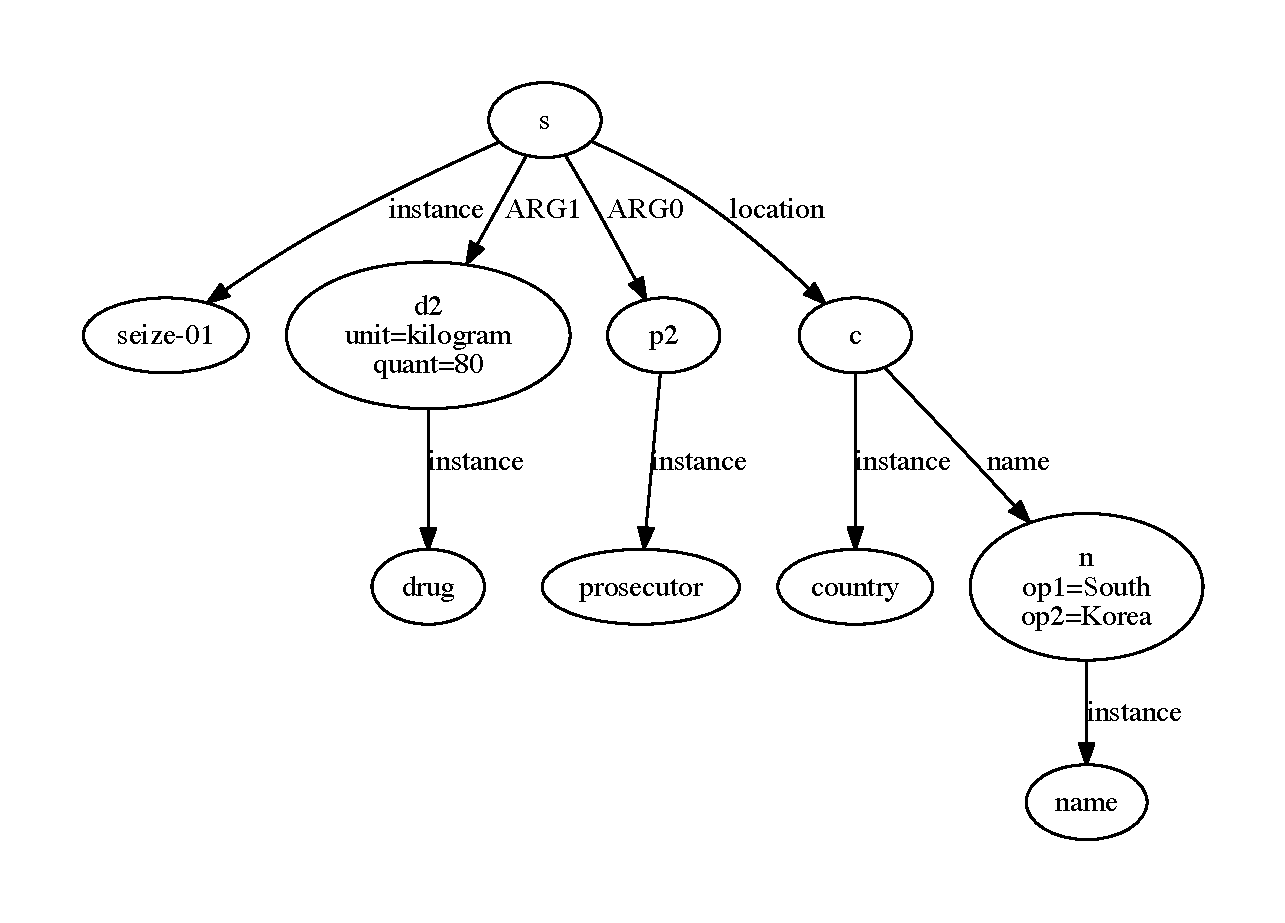
\includegraphics[width=\linewidth]{amr_example.pdf}
\caption{Example AMR}
\end{figure}

An AMR-annotated sentence is directed, rooted, labeled graph, or as a
conjunction of logical triples. Throughout this paper, we work with the AMRs
exclusively in the graphical form $G=(V,E)$, and will thus refer to the AMR
using just the sets $V,E$.

\subsection{Discourse Planning}

In Reiter and Dale's {\em Building Applied Natural Language Generation Systems}, they outline a 6-module pipeline for an NLG system. The second task in this system is Discourse Planning, which they describe as the process of imposing ordering and structure over the set of messages to be conveyed \cite{applied_nlg}. The order of pieces of information in text is not random; rather authors impose a structure on the messages for reasons such as: making the text easier to understand, highlighting the relationships between messages in the text, or stylistic preferences.When making an argument, authors must order the messages so that readers can see the logical implications from one message to the next; if the ordering of the messages were scrambled, readers may fail to understand the argument, even though the same set of information was communicated.

In addition to just logical implication, adjacent sentences can have many different types of relationships with each other, referred to as {\em discourse relations}. A commonly used set of discourse relations are those proposed by {\em Rhetorical Structure Theory} (RST) \cite{rst}. RST defines 32 discourse relations across 3 categories: ``Presentational Relations'', ``Subject Matter Relations'', and ``Multinuclear Relations''.

In applied systems, discourse planning is usually implemented through either schema-based systems or AI planning systems \cite{applied_nlg}. In schema-based systems, messages are given class labels, and are substituted into the appropriate slots which have been predefined in each schema. AI planning is a more general solution in which planning operators are associated with discourse relations, and then off-the-shelf planners can be used to construct a valid discourse plan \cite{hovy1993automated}\cite{paris1990natural}.

\subsection{Information Ordering}

Information ordering is an integral component of the Discourse Planning phase
of the NLG pipeline, discussed above and in \cite{applied_nlg}. After an
information set has been structured into to pieces of information (``facts" or
sentences), these pieces need to be ordered so that the reader can process and
understand the information being conveyed as easily as possible. This is often
approached as a planning problem, though Dimitromanolaki and
Androutsopoulos\cite{learning_to_order_facts} explore using pipelined decision
trees and instance-based learning.

\section{Related Work}

Early work by Kukich described a system for ``knowledge-based report generation'' in which manually specified domain rules were used to merge database facts into higher level messages, which were then ordered by a discourse module \cite{kukich1983knowledge}. The ordered output could later be passed to generation system to build a report. Work by Paris in 1990 and Hovy in 1993 introduced the idea of using AI Planners to generate discourse plans. They focused on finding explicit discourse relations between messages and using planners to generate an ordering which was allowed under the constraints of the discourse relations identified \cite{paris1990natural}\cite{hovy1993automated}. More recently, Duboue and Mckeown applied Machine Learning (ML) approaches to discourse planning. In \cite{duboue2001empirically}, they present an algorithm to learn ordering constraints among facts. In \cite{duboue2002content}, they build upon this work, using evolutionary algorithms to learn the tree representation of a planner. Although these systems seek to generate valid discourse plans, they do not use a scoring function to choose the `best' among the many valid plans that are available. Dimitromanolaki and Androutsopoulos used ML techniques to learn such a scoring function \cite{learning_to_order_facts}. They train a pipeline of classifiers that repeatedly choose the next fact to be added to a paragraph for a specific domain.
In order to train this pipeline, Dimitromanolaki and Androutsopoulos assume a
fixed $k$ number of sentences per paragraph (in their paper $k=6$).

Our work differs from this prior research in four major ways: (1) It is strictly at a semantic level. Our entire pipeline is built upon AMR semantics, rather than natural language `facts', meaning the internal entities and their relations can be reasoned about. (2) Higher-level messages are constructed as part of the discourse planning process. While other systems work at the individual fact level, our system seeks to group facts into higher level sentential messages that are ordered by our discourse module. The order of sentential units should be dependent on the information they contain, therefore the merging procedure must occur before or during the discourse planning. (3) Our system does not explicitly model the discourse relations between units.
(4) Our system imposes no limit on the number of sentences in a given
paragraph.

\section{Data}

\section{Preprocessing}
\subsection{ARG-of Reversal}
\subsection{Translation of `and' Semantics}
\subsection{Graph Merging}

\section{System Architecture}
\subsection{Subgraph Selection}
\subsection{Subgraph Ordering}

\section{Evaluation of Scoring Modules}
\subsection{Subgraph Selection}
\subsection{Subgraph Ordering}

\section{Experiments}

\section{Conclusion and Future Work}

\pagebreak
\bibliographystyle{acm}
\bibliography{paper}
\end{document}
